\documentclass[1p]{elsarticle_modified}
%\bibliographystyle{elsarticle-num}

%\usepackage[colorlinks]{hyperref}
%\usepackage{abbrmath_seonhwa} %\Abb, \Ascr, \Acal ,\Abf, \Afrak
\usepackage{amsfonts}
\usepackage{amssymb}
\usepackage{amsmath}
\usepackage{amsthm}
\usepackage{scalefnt}
\usepackage{amsbsy}
\usepackage{kotex}
\usepackage{caption}
\usepackage{subfig}
\usepackage{color}
\usepackage{graphicx}
\usepackage{xcolor} %% white, black, red, green, blue, cyan, magenta, yellow
\usepackage{float}
\usepackage{setspace}
\usepackage{hyperref}

\usepackage{tikz}
\usetikzlibrary{arrows}

\usepackage{multirow}
\usepackage{array} % fixed length table
\usepackage{hhline}

%%%%%%%%%%%%%%%%%%%%%
\makeatletter
\renewcommand*\env@matrix[1][\arraystretch]{%
	\edef\arraystretch{#1}%
	\hskip -\arraycolsep
	\let\@ifnextchar\new@ifnextchar
	\array{*\c@MaxMatrixCols c}}
\makeatother %https://tex.stackexchange.com/questions/14071/how-can-i-increase-the-line-spacing-in-a-matrix
%%%%%%%%%%%%%%%

\usepackage[normalem]{ulem}

\newcommand{\msout}[1]{\ifmmode\text{\sout{\ensuremath{#1}}}\else\sout{#1}\fi}
%SOURCE: \msout is \stkout macro in https://tex.stackexchange.com/questions/20609/strikeout-in-math-mode

\newcommand{\cancel}[1]{
	\ifmmode
	{\color{red}\msout{#1}}
	\else
	{\color{red}\sout{#1}}
	\fi
}

\newcommand{\add}[1]{
	{\color{blue}\uwave{#1}}
}

\newcommand{\replace}[2]{
	\ifmmode
	{\color{red}\msout{#1}}{\color{blue}\uwave{#2}}
	\else
	{\color{red}\sout{#1}}{\color{blue}\uwave{#2}}
	\fi
}

\newcommand{\Sol}{\mathcal{S}} %segment
\newcommand{\D}{D} %diagram
\newcommand{\A}{\mathcal{A}} %arc


%%%%%%%%%%%%%%%%%%%%%%%%%%%%%5 test

\def\sl{\operatorname{\textup{SL}}(2,\Cbb)}
\def\psl{\operatorname{\textup{PSL}}(2,\Cbb)}
\def\quan{\mkern 1mu \triangleright \mkern 1mu}

\theoremstyle{definition}
\newtheorem{thm}{Theorem}[section]
\newtheorem{prop}[thm]{Proposition}
\newtheorem{lem}[thm]{Lemma}
\newtheorem{ques}[thm]{Question}
\newtheorem{cor}[thm]{Corollary}
\newtheorem{defn}[thm]{Definition}
\newtheorem{exam}[thm]{Example}
\newtheorem{rmk}[thm]{Remark}
\newtheorem{alg}[thm]{Algorithm}

\newcommand{\I}{\sqrt{-1}}
\begin{document}

%\begin{frontmatter}
%
%\title{Boundary parabolic representations of knots up to 8 crossings}
%
%%% Group authors per affiliation:
%\author{Yunhi Cho} 
%\address{Department of Mathematics, University of Seoul, Seoul, Korea}
%\ead{yhcho@uos.ac.kr}
%
%
%\author{Seonhwa Kim} %\fnref{s_kim}}
%\address{Center for Geometry and Physics, Institute for Basic Science, Pohang, 37673, Korea}
%\ead{ryeona17@ibs.re.kr}
%
%\author{Hyuk Kim}
%\address{Department of Mathematical Sciences, Seoul National University, Seoul 08826, Korea}
%\ead{hyukkim@snu.ac.kr}
%
%\author{Seokbeom Yoon}
%\address{Department of Mathematical Sciences, Seoul National University, Seoul, 08826,  Korea}
%\ead{sbyoon15@snu.ac.kr}
%
%\begin{abstract}
%We find all boundary parabolic representation of knots up to 8 crossings.
%
%\end{abstract}
%\begin{keyword}
%    \MSC[2010] 57M25 
%\end{keyword}
%
%\end{frontmatter}

%\linenumbers
%\tableofcontents
%
\newcommand\colored[1]{\textcolor{white}{\rule[-0.35ex]{0.8em}{1.4ex}}\kern-0.8em\color{red} #1}%
%\newcommand\colored[1]{\textcolor{white}{ #1}\kern-2.17ex	\textcolor{white}{ #1}\kern-1.81ex	\textcolor{white}{ #1}\kern-2.15ex\color{red}#1	}

{\Large $\underline{12n_{0089}~(K12n_{0089})}$}

\setlength{\tabcolsep}{10pt}
\renewcommand{\arraystretch}{1.6}
\vspace{1cm}\begin{tabular}{m{100pt}>{\centering\arraybackslash}m{274pt}}
\multirow{5}{120pt}{
	\centering
	\includegraphics[width=112pt]{../../../GIT/diagram.site/Diagrams/png/2178_12n_0089.png}\\
\ \ \ A knot diagram\footnotemark}&
\allowdisplaybreaks
\textbf{Linearized knot diagam} \\
\cline{2-2}
 &
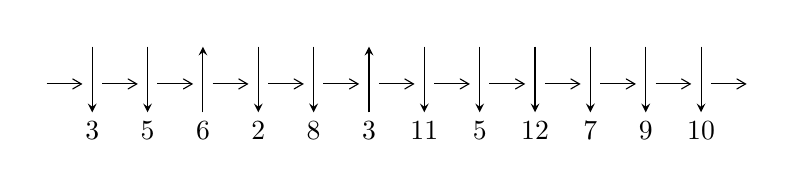
\begin{tikzpicture}[x=20pt, y=17pt]
	% nodes
	\node (C0) at (0, 0) {};
	\node (C1) at (1, 0) {};
	\node (C1U) at (1, +1) {};
	\node (C1D) at (1, -1) {3};

	\node (C2) at (2, 0) {};
	\node (C2U) at (2, +1) {};
	\node (C2D) at (2, -1) {5};

	\node (C3) at (3, 0) {};
	\node (C3U) at (3, +1) {};
	\node (C3D) at (3, -1) {6};

	\node (C4) at (4, 0) {};
	\node (C4U) at (4, +1) {};
	\node (C4D) at (4, -1) {2};

	\node (C5) at (5, 0) {};
	\node (C5U) at (5, +1) {};
	\node (C5D) at (5, -1) {8};

	\node (C6) at (6, 0) {};
	\node (C6U) at (6, +1) {};
	\node (C6D) at (6, -1) {3};

	\node (C7) at (7, 0) {};
	\node (C7U) at (7, +1) {};
	\node (C7D) at (7, -1) {11};

	\node (C8) at (8, 0) {};
	\node (C8U) at (8, +1) {};
	\node (C8D) at (8, -1) {5};

	\node (C9) at (9, 0) {};
	\node (C9U) at (9, +1) {};
	\node (C9D) at (9, -1) {12};

	\node (C10) at (10, 0) {};
	\node (C10U) at (10, +1) {};
	\node (C10D) at (10, -1) {7};

	\node (C11) at (11, 0) {};
	\node (C11U) at (11, +1) {};
	\node (C11D) at (11, -1) {9};

	\node (C12) at (12, 0) {};
	\node (C12U) at (12, +1) {};
	\node (C12D) at (12, -1) {10};
	\node (C13) at (13, 0) {};

	% arrows
	\draw[->,>={angle 60}]
	(C0) edge (C1) (C1) edge (C2) (C2) edge (C3) (C3) edge (C4) (C4) edge (C5) (C5) edge (C6) (C6) edge (C7) (C7) edge (C8) (C8) edge (C9) (C9) edge (C10) (C10) edge (C11) (C11) edge (C12) (C12) edge (C13) ;	\draw[->,>=stealth]
	(C1U) edge (C1D) (C2U) edge (C2D) (C3D) edge (C3U) (C4U) edge (C4D) (C5U) edge (C5D) (C6D) edge (C6U) (C7U) edge (C7D) (C8U) edge (C8D) (C9U) edge (C9D) (C10U) edge (C10D) (C11U) edge (C11D) (C12U) edge (C12D) ;
	\end{tikzpicture} \\
\hhline{~~} \\& 
\textbf{Solving Sequence} \\ \cline{2-2} 
 &
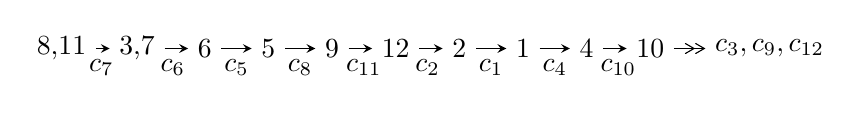
\begin{tikzpicture}[x=23pt, y=7pt]
	% node
	\node (A0) at (-1/8, 0) {8,11};
	\node (A1) at (17/16, 0) {3,7};
	\node (A2) at (17/8, 0) {6};
	\node (A3) at (25/8, 0) {5};
	\node (A4) at (33/8, 0) {9};
	\node (A5) at (41/8, 0) {12};
	\node (A6) at (49/8, 0) {2};
	\node (A7) at (57/8, 0) {1};
	\node (A8) at (65/8, 0) {4};
	\node (A9) at (73/8, 0) {10};
	\node (C1) at (1/2, -1) {$c_{7}$};
	\node (C2) at (13/8, -1) {$c_{6}$};
	\node (C3) at (21/8, -1) {$c_{5}$};
	\node (C4) at (29/8, -1) {$c_{8}$};
	\node (C5) at (37/8, -1) {$c_{11}$};
	\node (C6) at (45/8, -1) {$c_{2}$};
	\node (C7) at (53/8, -1) {$c_{1}$};
	\node (C8) at (61/8, -1) {$c_{4}$};
	\node (C9) at (69/8, -1) {$c_{10}$};
	\node (A10) at (11, 0) {$c_{3},c_{9},c_{12}$};

	% edge
	\draw[->,>=stealth]	
	(A0) edge (A1) (A1) edge (A2) (A2) edge (A3) (A3) edge (A4) (A4) edge (A5) (A5) edge (A6) (A6) edge (A7) (A7) edge (A8) (A8) edge (A9) ;
	\draw[->>,>={angle 60}]	
	(A9) edge (A10);
\end{tikzpicture} \\ 

\end{tabular} \\

\footnotetext{
The image of knot diagram is generated by the software ``\textbf{Draw programme}" developed by Andrew Bartholomew(\url{http://www.layer8.co.uk/maths/draw/index.htm\#Running-draw}), where we modified some parts for our purpose(\url{https://github.com/CATsTAILs/LinksPainter}).
}\phantom \\ \newline 
\centering \textbf{Ideals for irreducible components\footnotemark of $X_{\text{par}}$} 
 
\begin{align*}
I^u_{1}&=\langle 
1.87206\times10^{64} u^{33}-2.48020\times10^{64} u^{32}+\cdots+2.02349\times10^{64} b+8.89696\times10^{65},\\
\phantom{I^u_{1}}&\phantom{= \langle  }-6.94907\times10^{63} u^{33}+9.26153\times10^{63} u^{32}+\cdots+2.89069\times10^{63} a-3.41795\times10^{65},\\
\phantom{I^u_{1}}&\phantom{= \langle  }u^{34}-2 u^{33}+\cdots+160 u-32\rangle \\
I^u_{2}&=\langle 
-2 u^7+u^6+3 u^5-3 u^4-4 u^3+3 u^2+b+2 u-4,\;6 u^7-2 u^6-8 u^5+7 u^4+11 u^3-5 u^2+a-4 u+9,\\
\phantom{I^u_{2}}&\phantom{= \langle  }u^8- u^7- u^6+2 u^5+u^4-2 u^3+2 u-1\rangle \\
\\
I^v_{1}&=\langle 
a,\;-16 v^4-47 v^3-36 v^2+29 b-104 v+5,\;v^5+3 v^4+3 v^3+8 v^2+v+1\rangle \\
\end{align*}
\raggedright * 3 irreducible components of $\dim_{\mathbb{C}}=0$, with total 47 representations.\\
\footnotetext{All coefficients of polynomials are rational numbers. But the coefficients are sometimes approximated in decimal forms when there is not enough margin.}
\newpage
\renewcommand{\arraystretch}{1}
\centering \section*{I. $I^u_{1}= \langle 1.87\times10^{64} u^{33}-2.48\times10^{64} u^{32}+\cdots+2.02\times10^{64} b+8.90\times10^{65},\;-6.95\times10^{63} u^{33}+9.26\times10^{63} u^{32}+\cdots+2.89\times10^{63} a-3.42\times10^{65},\;u^{34}-2 u^{33}+\cdots+160 u-32 \rangle$}
\flushleft \textbf{(i) Arc colorings}\\
\begin{tabular}{m{7pt} m{180pt} m{7pt} m{180pt} }
\flushright $a_{8}=$&$\begin{pmatrix}1\\0\end{pmatrix}$ \\
\flushright $a_{11}=$&$\begin{pmatrix}0\\u\end{pmatrix}$ \\
\flushright $a_{3}=$&$\begin{pmatrix}2.40394 u^{33}-3.20391 u^{32}+\cdots-401.792 u+118.240\\-0.925166 u^{33}+1.22571 u^{32}+\cdots+151.603 u-43.9685\end{pmatrix}$ \\
\flushright $a_{7}=$&$\begin{pmatrix}1\\- u^2\end{pmatrix}$ \\
\flushright $a_{6}=$&$\begin{pmatrix}0.0490683 u^{33}-0.0407884 u^{32}+\cdots-6.92779 u+0.312774\\-0.0578563 u^{33}+0.0671443 u^{32}+\cdots+7.65767 u-1.83101\end{pmatrix}$ \\
\flushright $a_{5}=$&$\begin{pmatrix}-0.00878796 u^{33}+0.0263559 u^{32}+\cdots+0.729884 u-1.51823\\-0.0578563 u^{33}+0.0671443 u^{32}+\cdots+7.65767 u-1.83101\end{pmatrix}$ \\
\flushright $a_{9}=$&$\begin{pmatrix}0.135575 u^{33}-0.179353 u^{32}+\cdots-21.7295 u+6.37504\\-0.0869253 u^{33}+0.113172 u^{32}+\cdots+14.9258 u-4.00887\end{pmatrix}$ \\
\flushright $a_{12}=$&$\begin{pmatrix}-0.159247 u^{33}+0.209304 u^{32}+\cdots+26.3062 u-7.44642\\0.0515752 u^{33}-0.0698375 u^{32}+\cdots-7.79789 u+2.42273\end{pmatrix}$ \\
\flushright $a_{2}=$&$\begin{pmatrix}2.36320 u^{33}-3.16331 u^{32}+\cdots-395.428 u+117.533\\-0.844124 u^{33}+1.12821 u^{32}+\cdots+140.065 u-41.0098\end{pmatrix}$ \\
\flushright $a_{1}=$&$\begin{pmatrix}0.222500 u^{33}-0.292525 u^{32}+\cdots-36.6553 u+10.3839\\-0.0181808 u^{33}+0.0260797 u^{32}+\cdots+2.35027 u-0.870343\end{pmatrix}$ \\
\flushright $a_{4}=$&$\begin{pmatrix}2.25921 u^{33}-3.02557 u^{32}+\cdots-381.646 u+112.963\\-0.870163 u^{33}+1.15421 u^{32}+\cdots+144.300 u-42.2250\end{pmatrix}$ \\
\flushright $a_{10}=$&$\begin{pmatrix}u\\- u^3+u\end{pmatrix}$\\&\end{tabular}
\flushleft \textbf{(ii) Obstruction class $= -1$}\\~\\
\flushleft \textbf{(iii) Cusp Shapes $= -1.73770 u^{33}+2.33240 u^{32}+\cdots+305.829 u-87.7743$}\\~\\
\newpage\renewcommand{\arraystretch}{1}
\flushleft \textbf{(iv) u-Polynomials at the component}\newline \\
\begin{tabular}{m{50pt}|m{274pt}}
Crossings & \hspace{64pt}u-Polynomials at each crossing \\
\hline $$\begin{aligned}c_{1}\end{aligned}$$&$\begin{aligned}
&u^{34}+50 u^{33}+\cdots+7022 u+1
\end{aligned}$\\
\hline $$\begin{aligned}c_{2},c_{4}\end{aligned}$$&$\begin{aligned}
&u^{34}-10 u^{33}+\cdots-94 u+1
\end{aligned}$\\
\hline $$\begin{aligned}c_{3},c_{6}\end{aligned}$$&$\begin{aligned}
&u^{34}+6 u^{33}+\cdots+1408 u+256
\end{aligned}$\\
\hline $$\begin{aligned}c_{5},c_{8}\end{aligned}$$&$\begin{aligned}
&u^{34}-3 u^{33}+\cdots+2 u-1
\end{aligned}$\\
\hline $$\begin{aligned}c_{7},c_{10}\end{aligned}$$&$\begin{aligned}
&u^{34}+2 u^{33}+\cdots-160 u-32
\end{aligned}$\\
\hline $$\begin{aligned}c_{9},c_{11},c_{12}\end{aligned}$$&$\begin{aligned}
&u^{34}-7 u^{33}+\cdots+2 u+1
\end{aligned}$\\
\hline
\end{tabular}\\~\\
\newpage\renewcommand{\arraystretch}{1}
\flushleft \textbf{(v) Riley Polynomials at the component}\newline \\
\begin{tabular}{m{50pt}|m{274pt}}
Crossings & \hspace{64pt}Riley Polynomials at each crossing \\
\hline $$\begin{aligned}c_{1}\end{aligned}$$&$\begin{aligned}
&y^{34}-122 y^{33}+\cdots-49242950 y+1
\end{aligned}$\\
\hline $$\begin{aligned}c_{2},c_{4}\end{aligned}$$&$\begin{aligned}
&y^{34}-50 y^{33}+\cdots-7022 y+1
\end{aligned}$\\
\hline $$\begin{aligned}c_{3},c_{6}\end{aligned}$$&$\begin{aligned}
&y^{34}+54 y^{33}+\cdots-5357568 y+65536
\end{aligned}$\\
\hline $$\begin{aligned}c_{5},c_{8}\end{aligned}$$&$\begin{aligned}
&y^{34}- y^{33}+\cdots-14 y+1
\end{aligned}$\\
\hline $$\begin{aligned}c_{7},c_{10}\end{aligned}$$&$\begin{aligned}
&y^{34}-36 y^{33}+\cdots-3584 y+1024
\end{aligned}$\\
\hline $$\begin{aligned}c_{9},c_{11},c_{12}\end{aligned}$$&$\begin{aligned}
&y^{34}-41 y^{33}+\cdots-152 y+1
\end{aligned}$\\
\hline
\end{tabular}\\~\\
\newpage\flushleft \textbf{(vi) Complex Volumes and Cusp Shapes}
$$\begin{array}{c|c|c}  
\text{Solutions to }I^u_{1}& \I (\text{vol} + \sqrt{-1}CS) & \text{Cusp shape}\\
 \hline 
\begin{aligned}
u &= -0.956156 + 0.210490 I \\
a &= \phantom{-}0.92043 - 2.41941 I \\
b &= -0.297004 + 1.016390 I\end{aligned}
 & -3.57437 - 2.68652 I & -15.9734 + 5.7320 I \\ \hline\begin{aligned}
u &= -0.956156 - 0.210490 I \\
a &= \phantom{-}0.92043 + 2.41941 I \\
b &= -0.297004 - 1.016390 I\end{aligned}
 & -3.57437 + 2.68652 I & -15.9734 - 5.7320 I \\ \hline\begin{aligned}
u &= -0.825291 + 0.508770 I \\
a &= \phantom{-}0.290634 + 0.392014 I \\
b &= \phantom{-}0.215796 + 0.185230 I\end{aligned}
 & \phantom{-}1.50616 + 2.15286 I & -1.89528 - 3.55598 I \\ \hline\begin{aligned}
u &= -0.825291 - 0.508770 I \\
a &= \phantom{-}0.290634 - 0.392014 I \\
b &= \phantom{-}0.215796 - 0.185230 I\end{aligned}
 & \phantom{-}1.50616 - 2.15286 I & -1.89528 + 3.55598 I \\ \hline\begin{aligned}
u &= -0.459276 + 0.600077 I \\
a &= \phantom{-}0.34212 - 2.13952 I \\
b &= \phantom{-}0.325798 + 0.681195 I\end{aligned}
 & -4.37210 + 0.56022 I & -15.7627 - 4.5815 I \\ \hline\begin{aligned}
u &= -0.459276 - 0.600077 I \\
a &= \phantom{-}0.34212 + 2.13952 I \\
b &= \phantom{-}0.325798 - 0.681195 I\end{aligned}
 & -4.37210 - 0.56022 I & -15.7627 + 4.5815 I \\ \hline\begin{aligned}
u &= -1.25779\phantom{ +0.000000I} \\
a &= \phantom{-}0.262102\phantom{ +0.000000I} \\
b &= -0.999548\phantom{ +0.000000I}\end{aligned}
 & -7.19178\phantom{ +0.000000I} & -11.0680\phantom{ +0.000000I} \\ \hline\begin{aligned}
u &= \phantom{-}0.421643 + 0.589535 I \\
a &= \phantom{-}0.76749 - 1.22638 I \\
b &= -0.076416 - 0.398409 I\end{aligned}
 & -1.23502 + 0.89870 I & -5.08124 + 0.75731 I \\ \hline\begin{aligned}
u &= \phantom{-}0.421643 - 0.589535 I \\
a &= \phantom{-}0.76749 + 1.22638 I \\
b &= -0.076416 + 0.398409 I\end{aligned}
 & -1.23502 - 0.89870 I & -5.08124 - 0.75731 I \\ \hline\begin{aligned}
u &= \phantom{-}0.679857 + 0.008937 I \\
a &= \phantom{-}1.75490 - 5.31791 I \\
b &= -0.87873 + 2.06096 I\end{aligned}
 & -2.48043 + 0.15884 I & -35.3818 - 0.1674 I\\
 \hline 
 \end{array}$$\newpage$$\begin{array}{c|c|c}  
\text{Solutions to }I^u_{1}& \I (\text{vol} + \sqrt{-1}CS) & \text{Cusp shape}\\
 \hline 
\begin{aligned}
u &= \phantom{-}0.679857 - 0.008937 I \\
a &= \phantom{-}1.75490 + 5.31791 I \\
b &= -0.87873 - 2.06096 I\end{aligned}
 & -2.48043 - 0.15884 I & -35.3818 + 0.1674 I \\ \hline\begin{aligned}
u &= \phantom{-}1.204240 + 0.640025 I \\
a &= \phantom{-}0.153762 - 0.187566 I \\
b &= \phantom{-}0.460927 + 0.211334 I\end{aligned}
 & -3.73420 - 5.65524 I & -8.00000 + 0. I\phantom{ +0.000000I} \\ \hline\begin{aligned}
u &= \phantom{-}1.204240 - 0.640025 I \\
a &= \phantom{-}0.153762 + 0.187566 I \\
b &= \phantom{-}0.460927 - 0.211334 I\end{aligned}
 & -3.73420 + 5.65524 I & -8.00000 + 0. I\phantom{ +0.000000I} \\ \hline\begin{aligned}
u &= \phantom{-}0.610196\phantom{ +0.000000I} \\
a &= \phantom{-}0.685401\phantom{ +0.000000I} \\
b &= -0.364452\phantom{ +0.000000I}\end{aligned}
 & -0.859418\phantom{ +0.000000I} & -11.8170\phantom{ +0.000000I} \\ \hline\begin{aligned}
u &= -0.021309 + 0.580331 I \\
a &= \phantom{-}0.0854012 - 0.0908812 I \\
b &= -0.412066 + 1.299410 I\end{aligned}
 & -7.07612 - 4.33049 I & -3.74509 + 2.01968 I \\ \hline\begin{aligned}
u &= -0.021309 - 0.580331 I \\
a &= \phantom{-}0.0854012 + 0.0908812 I \\
b &= -0.412066 - 1.299410 I\end{aligned}
 & -7.07612 + 4.33049 I & -3.74509 - 2.01968 I \\ \hline\begin{aligned}
u &= \phantom{-}0.033914 + 0.417650 I \\
a &= \phantom{-}0.837170 - 0.008519 I \\
b &= \phantom{-}0.336239 - 0.914967 I\end{aligned}
 & -0.57544 - 1.50411 I & -4.52476 + 4.55824 I \\ \hline\begin{aligned}
u &= \phantom{-}0.033914 - 0.417650 I \\
a &= \phantom{-}0.837170 + 0.008519 I \\
b &= \phantom{-}0.336239 + 0.914967 I\end{aligned}
 & -0.57544 + 1.50411 I & -4.52476 - 4.55824 I \\ \hline\begin{aligned}
u &= \phantom{-}0.333190\phantom{ +0.000000I} \\
a &= \phantom{-}5.02872\phantom{ +0.000000I} \\
b &= -1.11629\phantom{ +0.000000I}\end{aligned}
 & -2.28474\phantom{ +0.000000I} & \phantom{-}0.324850\phantom{ +0.000000I} \\ \hline\begin{aligned}
u &= -1.71423 + 0.26922 I \\
a &= \phantom{-}0.105003 - 1.399260 I \\
b &= \phantom{-}0.34011 + 1.96867 I\end{aligned}
 & -13.7038 + 7.6996 I & \phantom{-0.000000 } 0\\
 \hline 
 \end{array}$$\newpage$$\begin{array}{c|c|c}  
\text{Solutions to }I^u_{1}& \I (\text{vol} + \sqrt{-1}CS) & \text{Cusp shape}\\
 \hline 
\begin{aligned}
u &= -1.71423 - 0.26922 I \\
a &= \phantom{-}0.105003 + 1.399260 I \\
b &= \phantom{-}0.34011 - 1.96867 I\end{aligned}
 & -13.7038 - 7.6996 I & \phantom{-0.000000 } 0 \\ \hline\begin{aligned}
u &= \phantom{-}1.71822 + 0.31095 I \\
a &= -0.469943 - 1.223830 I \\
b &= -0.06244 + 1.83419 I\end{aligned}
 & -13.63590 + 0.50051 I & \phantom{-0.000000 } 0 \\ \hline\begin{aligned}
u &= \phantom{-}1.71822 - 0.31095 I \\
a &= -0.469943 + 1.223830 I \\
b &= -0.06244 - 1.83419 I\end{aligned}
 & -13.63590 - 0.50051 I & \phantom{-0.000000 } 0 \\ \hline\begin{aligned}
u &= -1.74355 + 0.15186 I \\
a &= \phantom{-}0.014975 - 1.244930 I \\
b &= \phantom{-}1.07725 + 2.72182 I\end{aligned}
 & -10.90540 + 1.31562 I & \phantom{-0.000000 } 0 \\ \hline\begin{aligned}
u &= -1.74355 - 0.15186 I \\
a &= \phantom{-}0.014975 + 1.244930 I \\
b &= \phantom{-}1.07725 - 2.72182 I\end{aligned}
 & -10.90540 - 1.31562 I & \phantom{-0.000000 } 0 \\ \hline\begin{aligned}
u &= -0.01973 + 1.82329 I \\
a &= \phantom{-}0.0829691 + 0.0828182 I \\
b &= -0.11557 - 1.98219 I\end{aligned}
 & -16.1286 + 4.0950 I & \phantom{-0.000000 } 0 \\ \hline\begin{aligned}
u &= -0.01973 - 1.82329 I \\
a &= \phantom{-}0.0829691 - 0.0828182 I \\
b &= -0.11557 + 1.98219 I\end{aligned}
 & -16.1286 - 4.0950 I & \phantom{-0.000000 } 0 \\ \hline\begin{aligned}
u &= \phantom{-}1.85359 + 0.31631 I \\
a &= -0.231341 - 1.229070 I \\
b &= -0.48186 + 1.53845 I\end{aligned}
 & -12.71500 - 5.35446 I & \phantom{-0.000000 } 0 \\ \hline\begin{aligned}
u &= \phantom{-}1.85359 - 0.31631 I \\
a &= -0.231341 + 1.229070 I \\
b &= -0.48186 - 1.53845 I\end{aligned}
 & -12.71500 + 5.35446 I & \phantom{-0.000000 } 0 \\ \hline\begin{aligned}
u &= \phantom{-}1.72228 + 0.86852 I \\
a &= \phantom{-}0.576188 + 1.082400 I \\
b &= \phantom{-}0.76478 - 2.07350 I\end{aligned}
 & \phantom{-}18.1726 - 13.4286 I & \phantom{-0.000000 } 0\\
 \hline 
 \end{array}$$\newpage$$\begin{array}{c|c|c}  
\text{Solutions to }I^u_{1}& \I (\text{vol} + \sqrt{-1}CS) & \text{Cusp shape}\\
 \hline 
\begin{aligned}
u &= \phantom{-}1.72228 - 0.86852 I \\
a &= \phantom{-}0.576188 - 1.082400 I \\
b &= \phantom{-}0.76478 + 2.07350 I\end{aligned}
 & \phantom{-}18.1726 + 13.4286 I & \phantom{-0.000000 } 0 \\ \hline\begin{aligned}
u &= -1.71660 + 0.90954 I \\
a &= -0.667196 + 0.794326 I \\
b &= -0.51034 - 1.64958 I\end{aligned}
 & \phantom{-}18.3538 + 5.3451 I & \phantom{-0.000000 } 0 \\ \hline\begin{aligned}
u &= -1.71660 - 0.90954 I \\
a &= -0.667196 - 0.794326 I \\
b &= -0.51034 + 1.64958 I\end{aligned}
 & \phantom{-}18.3538 - 5.3451 I & \phantom{-0.000000 } 0 \\ \hline\begin{aligned}
u &= \phantom{-}1.95923\phantom{ +0.000000I} \\
a &= -0.601374\phantom{ +0.000000I} \\
b &= -0.892648\phantom{ +0.000000I}\end{aligned}
 & -15.4063\phantom{ +0.000000I} & \phantom{-0.000000 } 0\\
 \hline 
 \end{array}$$\newpage\newpage\renewcommand{\arraystretch}{1}
\centering \section*{II. $I^u_{2}= \langle -2 u^7+u^6+\cdots+b-4,\;6 u^7-2 u^6+\cdots+a+9,\;u^8- u^7- u^6+2 u^5+u^4-2 u^3+2 u-1 \rangle$}
\flushleft \textbf{(i) Arc colorings}\\
\begin{tabular}{m{7pt} m{180pt} m{7pt} m{180pt} }
\flushright $a_{8}=$&$\begin{pmatrix}1\\0\end{pmatrix}$ \\
\flushright $a_{11}=$&$\begin{pmatrix}0\\u\end{pmatrix}$ \\
\flushright $a_{3}=$&$\begin{pmatrix}-6 u^7+2 u^6+8 u^5-7 u^4-11 u^3+5 u^2+4 u-9\\2 u^7- u^6-3 u^5+3 u^4+4 u^3-3 u^2-2 u+4\end{pmatrix}$ \\
\flushright $a_{7}=$&$\begin{pmatrix}1\\- u^2\end{pmatrix}$ \\
\flushright $a_{6}=$&$\begin{pmatrix}1\\- u^2\end{pmatrix}$ \\
\flushright $a_{5}=$&$\begin{pmatrix}- u^2+1\\- u^2\end{pmatrix}$ \\
\flushright $a_{9}=$&$\begin{pmatrix}u^4- u^2+1\\u^4\end{pmatrix}$ \\
\flushright $a_{12}=$&$\begin{pmatrix}u^6- u^4+2 u^2-1\\- u^7+u^6+2 u^5- u^4-2 u^3+2 u^2+2 u-1\end{pmatrix}$ \\
\flushright $a_{2}=$&$\begin{pmatrix}-6 u^7+2 u^6+8 u^5-7 u^4-11 u^3+6 u^2+4 u-10\\2 u^7- u^6-3 u^5+3 u^4+4 u^3-2 u^2-2 u+4\end{pmatrix}$ \\
\flushright $a_{1}=$&$\begin{pmatrix}u^2-1\\u^2\end{pmatrix}$ \\
\flushright $a_{4}=$&$\begin{pmatrix}-6 u^7+2 u^6+8 u^5-7 u^4-11 u^3+5 u^2+4 u-9\\2 u^7- u^6-3 u^5+3 u^4+4 u^3-3 u^2-2 u+4\end{pmatrix}$ \\
\flushright $a_{10}=$&$\begin{pmatrix}u\\- u^3+u\end{pmatrix}$\\&\end{tabular}
\flushleft \textbf{(ii) Obstruction class $= 1$}\\~\\
\flushleft \textbf{(iii) Cusp Shapes $= -44 u^7+15 u^6+58 u^5-53 u^4-78 u^3+42 u^2+28 u-85$}\\~\\
\newpage\renewcommand{\arraystretch}{1}
\flushleft \textbf{(iv) u-Polynomials at the component}\newline \\
\begin{tabular}{m{50pt}|m{274pt}}
Crossings & \hspace{64pt}u-Polynomials at each crossing \\
\hline $$\begin{aligned}c_{1},c_{2}\end{aligned}$$&$\begin{aligned}
&(u-1)^8
\end{aligned}$\\
\hline $$\begin{aligned}c_{3},c_{6}\end{aligned}$$&$\begin{aligned}
&u^8
\end{aligned}$\\
\hline $$\begin{aligned}c_{4}\end{aligned}$$&$\begin{aligned}
&(u+1)^8
\end{aligned}$\\
\hline $$\begin{aligned}c_{5}\end{aligned}$$&$\begin{aligned}
&u^8-3 u^7+7 u^6-10 u^5+11 u^4-10 u^3+6 u^2-4 u+1
\end{aligned}$\\
\hline $$\begin{aligned}c_{7}\end{aligned}$$&$\begin{aligned}
&u^8- u^7- u^6+2 u^5+u^4-2 u^3+2 u-1
\end{aligned}$\\
\hline $$\begin{aligned}c_{8}\end{aligned}$$&$\begin{aligned}
&u^8+3 u^7+7 u^6+10 u^5+11 u^4+10 u^3+6 u^2+4 u+1
\end{aligned}$\\
\hline $$\begin{aligned}c_{9}\end{aligned}$$&$\begin{aligned}
&u^8+u^7-3 u^6-2 u^5+3 u^4+2 u-1
\end{aligned}$\\
\hline $$\begin{aligned}c_{10}\end{aligned}$$&$\begin{aligned}
&u^8+u^7- u^6-2 u^5+u^4+2 u^3-2 u-1
\end{aligned}$\\
\hline $$\begin{aligned}c_{11},c_{12}\end{aligned}$$&$\begin{aligned}
&u^8- u^7-3 u^6+2 u^5+3 u^4-2 u-1
\end{aligned}$\\
\hline
\end{tabular}\\~\\
\newpage\renewcommand{\arraystretch}{1}
\flushleft \textbf{(v) Riley Polynomials at the component}\newline \\
\begin{tabular}{m{50pt}|m{274pt}}
Crossings & \hspace{64pt}Riley Polynomials at each crossing \\
\hline $$\begin{aligned}c_{1},c_{2},c_{4}\end{aligned}$$&$\begin{aligned}
&(y-1)^8
\end{aligned}$\\
\hline $$\begin{aligned}c_{3},c_{6}\end{aligned}$$&$\begin{aligned}
&y^8
\end{aligned}$\\
\hline $$\begin{aligned}c_{5},c_{8}\end{aligned}$$&$\begin{aligned}
&y^8+5 y^7+11 y^6+6 y^5-17 y^4-34 y^3-22 y^2-4 y+1
\end{aligned}$\\
\hline $$\begin{aligned}c_{7},c_{10}\end{aligned}$$&$\begin{aligned}
&y^8-3 y^7+7 y^6-10 y^5+11 y^4-10 y^3+6 y^2-4 y+1
\end{aligned}$\\
\hline $$\begin{aligned}c_{9},c_{11},c_{12}\end{aligned}$$&$\begin{aligned}
&y^8-7 y^7+19 y^6-22 y^5+3 y^4+14 y^3-6 y^2-4 y+1
\end{aligned}$\\
\hline
\end{tabular}\\~\\
\newpage\flushleft \textbf{(vi) Complex Volumes and Cusp Shapes}
$$\begin{array}{c|c|c}  
\text{Solutions to }I^u_{2}& \I (\text{vol} + \sqrt{-1}CS) & \text{Cusp shape}\\
 \hline 
\begin{aligned}
u &= \phantom{-}0.570868 + 0.730671 I \\
a &= \phantom{-}1.194470 - 0.635084 I \\
b &= -0.281371 - 1.128550 I\end{aligned}
 & -2.68559 + 1.13123 I & -12.74421 + 0.55338 I \\ \hline\begin{aligned}
u &= \phantom{-}0.570868 - 0.730671 I \\
a &= \phantom{-}1.194470 + 0.635084 I \\
b &= -0.281371 + 1.128550 I\end{aligned}
 & -2.68559 - 1.13123 I & -12.74421 - 0.55338 I \\ \hline\begin{aligned}
u &= -0.855237 + 0.665892 I \\
a &= \phantom{-}0.637416 - 0.344390 I \\
b &= \phantom{-}0.208670 + 0.825203 I\end{aligned}
 & \phantom{-}0.51448 + 2.57849 I & -9.60894 - 4.72239 I \\ \hline\begin{aligned}
u &= -0.855237 - 0.665892 I \\
a &= \phantom{-}0.637416 + 0.344390 I \\
b &= \phantom{-}0.208670 - 0.825203 I\end{aligned}
 & \phantom{-}0.51448 - 2.57849 I & -9.60894 + 4.72239 I \\ \hline\begin{aligned}
u &= -1.09818\phantom{ +0.000000I} \\
a &= -0.687555\phantom{ +0.000000I} \\
b &= \phantom{-}0.829189\phantom{ +0.000000I}\end{aligned}
 & -8.14766\phantom{ +0.000000I} & -20.4520\phantom{ +0.000000I} \\ \hline\begin{aligned}
u &= \phantom{-}1.031810 + 0.655470 I \\
a &= \phantom{-}0.286111 + 0.344558 I \\
b &= \phantom{-}0.284386 - 0.605794 I\end{aligned}
 & -4.02461 - 6.44354 I & -12.4754 + 9.9976 I \\ \hline\begin{aligned}
u &= \phantom{-}1.031810 - 0.655470 I \\
a &= \phantom{-}0.286111 - 0.344558 I \\
b &= \phantom{-}0.284386 + 0.605794 I\end{aligned}
 & -4.02461 + 6.44354 I & -12.4754 - 9.9976 I \\ \hline\begin{aligned}
u &= \phantom{-}0.603304\phantom{ +0.000000I} \\
a &= -7.54843\phantom{ +0.000000I} \\
b &= \phantom{-}2.74744\phantom{ +0.000000I}\end{aligned}
 & -2.48997\phantom{ +0.000000I} & -72.8910\phantom{ +0.000000I}\\
 \hline 
 \end{array}$$\newpage\newpage\renewcommand{\arraystretch}{1}
\centering \section*{III. $I^v_{1}= \langle a,\;-16 v^4-47 v^3-36 v^2+29 b-104 v+5,\;v^5+3 v^4+3 v^3+8 v^2+v+1 \rangle$}
\flushleft \textbf{(i) Arc colorings}\\
\begin{tabular}{m{7pt} m{180pt} m{7pt} m{180pt} }
\flushright $a_{8}=$&$\begin{pmatrix}1\\0\end{pmatrix}$ \\
\flushright $a_{11}=$&$\begin{pmatrix}v\\0\end{pmatrix}$ \\
\flushright $a_{3}=$&$\begin{pmatrix}0\\0.551724 v^{4}+1.62069 v^{3}+\cdots+3.58621 v-0.172414\end{pmatrix}$ \\
\flushright $a_{7}=$&$\begin{pmatrix}1\\0\end{pmatrix}$ \\
\flushright $a_{6}=$&$\begin{pmatrix}1\\-0.344828 v^{4}-1.13793 v^{3}+\cdots-3.24138 v-1.51724\end{pmatrix}$ \\
\flushright $a_{5}=$&$\begin{pmatrix}-0.344828 v^{4}-1.13793 v^{3}+\cdots-3.24138 v-0.517241\\-0.344828 v^{4}-1.13793 v^{3}+\cdots-3.24138 v-1.51724\end{pmatrix}$ \\
\flushright $a_{9}=$&$\begin{pmatrix}0.655172 v^{4}+1.86207 v^{3}+\cdots+4.75862 v+0.482759\\v^4+3 v^3+3 v^2+8 v+1\end{pmatrix}$ \\
\flushright $a_{12}=$&$\begin{pmatrix}-0.655172 v^{4}-1.86207 v^{3}+\cdots-3.75862 v-0.482759\\- v^4-3 v^3-3 v^2-8 v-1\end{pmatrix}$ \\
\flushright $a_{2}=$&$\begin{pmatrix}-0.655172 v^{4}-1.86207 v^{3}+\cdots-4.75862 v-0.482759\\-0.137931 v^{4}-0.655172 v^{3}+\cdots-1.89655 v-2.20690\end{pmatrix}$ \\
\flushright $a_{1}=$&$\begin{pmatrix}-0.655172 v^{4}-1.86207 v^{3}+\cdots-4.75862 v-0.482759\\- v^4-3 v^3-3 v^2-8 v-1\end{pmatrix}$ \\
\flushright $a_{4}=$&$\begin{pmatrix}0.551724 v^{4}+1.62069 v^{3}+\cdots+3.58621 v-0.172414\\0.0344828 v^{4}+0.413793 v^{3}+\cdots+0.724138 v+1.55172\end{pmatrix}$ \\
\flushright $a_{10}=$&$\begin{pmatrix}v\\0\end{pmatrix}$\\&\end{tabular}
\flushleft \textbf{(ii) Obstruction class $= 1$}\\~\\
\flushleft \textbf{(iii) Cusp Shapes $= \frac{65}{29} v^4+\frac{142}{29} v^3+\frac{81}{29} v^2+\frac{437}{29} v-\frac{613}{29}$}\\~\\
\newpage\renewcommand{\arraystretch}{1}
\flushleft \textbf{(iv) u-Polynomials at the component}\newline \\
\begin{tabular}{m{50pt}|m{274pt}}
Crossings & \hspace{64pt}u-Polynomials at each crossing \\
\hline $$\begin{aligned}c_{1}\end{aligned}$$&$\begin{aligned}
&u^5-5 u^4+8 u^3-3 u^2- u-1
\end{aligned}$\\
\hline $$\begin{aligned}c_{2}\end{aligned}$$&$\begin{aligned}
&u^5+u^4-2 u^3- u^2+u-1
\end{aligned}$\\
\hline $$\begin{aligned}c_{3}\end{aligned}$$&$\begin{aligned}
&u^5- u^4+2 u^3- u^2+u-1
\end{aligned}$\\
\hline $$\begin{aligned}c_{4}\end{aligned}$$&$\begin{aligned}
&u^5- u^4-2 u^3+u^2+u+1
\end{aligned}$\\
\hline $$\begin{aligned}c_{5}\end{aligned}$$&$\begin{aligned}
&u^5-3 u^4+4 u^3- u^2- u+1
\end{aligned}$\\
\hline $$\begin{aligned}c_{6}\end{aligned}$$&$\begin{aligned}
&u^5+u^4+2 u^3+u^2+u+1
\end{aligned}$\\
\hline $$\begin{aligned}c_{7},c_{10}\end{aligned}$$&$\begin{aligned}
&u^5
\end{aligned}$\\
\hline $$\begin{aligned}c_{8}\end{aligned}$$&$\begin{aligned}
&u^5+3 u^4+4 u^3+u^2- u-1
\end{aligned}$\\
\hline $$\begin{aligned}c_{9}\end{aligned}$$&$\begin{aligned}
&(u-1)^5
\end{aligned}$\\
\hline $$\begin{aligned}c_{11},c_{12}\end{aligned}$$&$\begin{aligned}
&(u+1)^5
\end{aligned}$\\
\hline
\end{tabular}\\~\\
\newpage\renewcommand{\arraystretch}{1}
\flushleft \textbf{(v) Riley Polynomials at the component}\newline \\
\begin{tabular}{m{50pt}|m{274pt}}
Crossings & \hspace{64pt}Riley Polynomials at each crossing \\
\hline $$\begin{aligned}c_{1}\end{aligned}$$&$\begin{aligned}
&y^5-9 y^4+32 y^3-35 y^2-5 y-1
\end{aligned}$\\
\hline $$\begin{aligned}c_{2},c_{4}\end{aligned}$$&$\begin{aligned}
&y^5-5 y^4+8 y^3-3 y^2- y-1
\end{aligned}$\\
\hline $$\begin{aligned}c_{3},c_{6}\end{aligned}$$&$\begin{aligned}
&y^5+3 y^4+4 y^3+y^2- y-1
\end{aligned}$\\
\hline $$\begin{aligned}c_{5},c_{8}\end{aligned}$$&$\begin{aligned}
&y^5- y^4+8 y^3-3 y^2+3 y-1
\end{aligned}$\\
\hline $$\begin{aligned}c_{7},c_{10}\end{aligned}$$&$\begin{aligned}
&y^5
\end{aligned}$\\
\hline $$\begin{aligned}c_{9},c_{11},c_{12}\end{aligned}$$&$\begin{aligned}
&(y-1)^5
\end{aligned}$\\
\hline
\end{tabular}\\~\\
\newpage\flushleft \textbf{(vi) Complex Volumes and Cusp Shapes}
$$\begin{array}{c|c|c}  
\text{Solutions to }I^v_{1}& \I (\text{vol} + \sqrt{-1}CS) & \text{Cusp shape}\\
 \hline 
\begin{aligned}
v &= -0.01014 + 1.59703 I \\
a &= \phantom{-0.000000 } 0 \\
b &= \phantom{-}0.339110 - 0.822375 I\end{aligned}
 & -1.97403 - 1.53058 I & -13.4575 + 4.4032 I \\ \hline\begin{aligned}
v &= -0.01014 - 1.59703 I \\
a &= \phantom{-0.000000 } 0 \\
b &= \phantom{-}0.339110 + 0.822375 I\end{aligned}
 & -1.97403 + 1.53058 I & -13.4575 - 4.4032 I \\ \hline\begin{aligned}
v &= -0.043806 + 0.365575 I \\
a &= \phantom{-0.000000 } 0 \\
b &= -0.455697 + 1.200150 I\end{aligned}
 & -7.51750 - 4.40083 I & -22.0438 + 5.2094 I \\ \hline\begin{aligned}
v &= -0.043806 - 0.365575 I \\
a &= \phantom{-0.000000 } 0 \\
b &= -0.455697 - 1.200150 I\end{aligned}
 & -7.51750 + 4.40083 I & -22.0438 - 5.2094 I \\ \hline\begin{aligned}
v &= -2.89210\phantom{ +0.000000I} \\
a &= \phantom{-0.000000 } 0 \\
b &= -0.766826\phantom{ +0.000000I}\end{aligned}
 & -4.04602\phantom{ +0.000000I} & -2.99730\phantom{ +0.000000I}\\
 \hline 
 \end{array}$$\newpage
\newpage\renewcommand{\arraystretch}{1}
\centering \section*{ IV. u-Polynomials}
\begin{tabular}{m{50pt}|m{274pt}}
Crossings & \hspace{64pt}u-Polynomials at each crossing \\
\hline $$\begin{aligned}c_{1}\end{aligned}$$&$\begin{aligned}
&((u-1)^8)(u^5-5 u^4+\cdots- u-1)(u^{34}+50 u^{33}+\cdots+7022 u+1)
\end{aligned}$\\
\hline $$\begin{aligned}c_{2}\end{aligned}$$&$\begin{aligned}
&((u-1)^8)(u^5+u^4+\cdots+u-1)(u^{34}-10 u^{33}+\cdots-94 u+1)
\end{aligned}$\\
\hline $$\begin{aligned}c_{3}\end{aligned}$$&$\begin{aligned}
&u^8(u^5- u^4+\cdots+u-1)(u^{34}+6 u^{33}+\cdots+1408 u+256)
\end{aligned}$\\
\hline $$\begin{aligned}c_{4}\end{aligned}$$&$\begin{aligned}
&((u+1)^8)(u^5- u^4+\cdots+u+1)(u^{34}-10 u^{33}+\cdots-94 u+1)
\end{aligned}$\\
\hline $$\begin{aligned}c_{5}\end{aligned}$$&$\begin{aligned}
&(u^5-3 u^4+4 u^3- u^2- u+1)\\
&\cdot(u^8-3 u^7+7 u^6-10 u^5+11 u^4-10 u^3+6 u^2-4 u+1)\\
&\cdot(u^{34}-3 u^{33}+\cdots+2 u-1)
\end{aligned}$\\
\hline $$\begin{aligned}c_{6}\end{aligned}$$&$\begin{aligned}
&u^8(u^5+u^4+\cdots+u+1)(u^{34}+6 u^{33}+\cdots+1408 u+256)
\end{aligned}$\\
\hline $$\begin{aligned}c_{7}\end{aligned}$$&$\begin{aligned}
&u^5(u^8- u^7+\cdots+2 u-1)(u^{34}+2 u^{33}+\cdots-160 u-32)
\end{aligned}$\\
\hline $$\begin{aligned}c_{8}\end{aligned}$$&$\begin{aligned}
&(u^5+3 u^4+4 u^3+u^2- u-1)\\
&\cdot(u^8+3 u^7+7 u^6+10 u^5+11 u^4+10 u^3+6 u^2+4 u+1)\\
&\cdot(u^{34}-3 u^{33}+\cdots+2 u-1)
\end{aligned}$\\
\hline $$\begin{aligned}c_{9}\end{aligned}$$&$\begin{aligned}
&((u-1)^5)(u^8+u^7+\cdots+2 u-1)(u^{34}-7 u^{33}+\cdots+2 u+1)
\end{aligned}$\\
\hline $$\begin{aligned}c_{10}\end{aligned}$$&$\begin{aligned}
&u^5(u^8+u^7+\cdots-2 u-1)(u^{34}+2 u^{33}+\cdots-160 u-32)
\end{aligned}$\\
\hline $$\begin{aligned}c_{11},c_{12}\end{aligned}$$&$\begin{aligned}
&((u+1)^5)(u^8- u^7+\cdots-2 u-1)(u^{34}-7 u^{33}+\cdots+2 u+1)
\end{aligned}$\\
\hline
\end{tabular}\newpage\renewcommand{\arraystretch}{1}
\centering \section*{ V. Riley Polynomials}
\begin{tabular}{m{50pt}|m{274pt}}
Crossings & \hspace{64pt}Riley Polynomials at each crossing \\
\hline $$\begin{aligned}c_{1}\end{aligned}$$&$\begin{aligned}
&(y-1)^8(y^5-9 y^4+32 y^3-35 y^2-5 y-1)\\
&\cdot(y^{34}-122 y^{33}+\cdots-49242950 y+1)
\end{aligned}$\\
\hline $$\begin{aligned}c_{2},c_{4}\end{aligned}$$&$\begin{aligned}
&((y-1)^8)(y^5-5 y^4+\cdots- y-1)(y^{34}-50 y^{33}+\cdots-7022 y+1)
\end{aligned}$\\
\hline $$\begin{aligned}c_{3},c_{6}\end{aligned}$$&$\begin{aligned}
&y^8(y^5+3 y^4+\cdots- y-1)(y^{34}+54 y^{33}+\cdots-5357568 y+65536)
\end{aligned}$\\
\hline $$\begin{aligned}c_{5},c_{8}\end{aligned}$$&$\begin{aligned}
&(y^5- y^4+8 y^3-3 y^2+3 y-1)\\
&\cdot(y^8+5 y^7+11 y^6+6 y^5-17 y^4-34 y^3-22 y^2-4 y+1)\\
&\cdot(y^{34}- y^{33}+\cdots-14 y+1)
\end{aligned}$\\
\hline $$\begin{aligned}c_{7},c_{10}\end{aligned}$$&$\begin{aligned}
&y^5(y^8-3 y^7+7 y^6-10 y^5+11 y^4-10 y^3+6 y^2-4 y+1)\\
&\cdot(y^{34}-36 y^{33}+\cdots-3584 y+1024)
\end{aligned}$\\
\hline $$\begin{aligned}c_{9},c_{11},c_{12}\end{aligned}$$&$\begin{aligned}
&(y-1)^5(y^8-7 y^7+19 y^6-22 y^5+3 y^4+14 y^3-6 y^2-4 y+1)\\
&\cdot(y^{34}-41 y^{33}+\cdots-152 y+1)
\end{aligned}$\\
\hline
\end{tabular}
\vskip 2pc
\end{document}